%%% Ch. 5: Discussion & Analysis%%%
\chapter{Discussion \& Analysis} \label{ch:discussion}
The endorsement system provides a method to assign a global trust score to the
participants of the endorsement network. The \ac{TEI} score represents the
impact a node has made on the network by sending or receiving endorsements.
Based on this score, one can infer the trustworthiness of an entity. Discussion
of several possible threats that can exist in a trust and reputation system
along with how the endorsement model addresses them is presented by
Chapter~\ref{ch:results}. The issues that a reputation system should address
based on principles defined by EigenTrust~\cite{kamvar2003eigentrust} and
Resnick et. al~\cite{resnick2000reputation} are discussed by the design
considerations in Section~\ref{subsec:designconsiderations} and taken into
account by the endorsement model. To briefly summarize each of them:  

\paragraph{Self-policing:}By deploying a decentralized endorsement system on a
public permission-less blockchain network and allowing anyone to execute the
contract code and change the contract's state by performing endorsement
interactions, the role of a trusted central entity is removed. The
specifications of user interaction and the method to compute the trust score
are defined by the smart contract. As such, the peers in the endorsement system
are responsible for writing or modifying the reputation data that complies with
the specified logic.   
\paragraph{Anonymity:} The reputation of a peer is associated with the public
key hash of the account, i.e., the account identifier and not with the
externally associated identity such as their IP address or a government-issued
identity.  
\paragraph{No profit to newcomers:}As illustrated by Section~\ref{par:TEI} in
Chapter~\ref{ch:results}, the starting node cannot have a significant impact
value right away. They start with an ignorant value (i.e., 0) and it takes more
than one endorsement interactions (incoming and outgoing) to be considered for
the computation of \ac{TEI}. After which, it takes several incoming and
outgoing endorsement connections along with maintenance of several factors
(i.e., ratio, \ac{TRP}) to make a significant impact on the network. Thus, the
model addresses the issue of "no profit to newcomers". Apart from these
factors, the notion of punishment as discussed earlier ensures that there is no
profit in joining as a newcomer by leaving the network as a non-reputable
account.   
\paragraph{Minimal Overhead:}This relates to minimal overhead in terms of
storage, computation, infrastructure and message complexity. Thus, this factor
is directly related to Ethereum as infrastructure and the execution of the
endorsement contract on the blockchain. There is no limit to the length of data
a transaction message (e.g., computation of \ac{TEI}) can hold but more data
implies more gas fee since the amount of storage that every node (full nodes)
have to store increases. The cost of transaction fee is paid by the account
that initiates the transaction. The transaction fee for the endorsement is
associated with the update and storage operation. Sending an endorsement to
another account updates the state variables \ac{nEG} and \ac{nER} and stores
the new endorser and endorsee address for the respective accounts. The
computation of total endorsement impact for a given entity $A$ can be initiated
by any node (not just the account owner). This computation step depends on the
size of the endorsee array of $A$. As discussed in
Section~\ref{subsec:datablockchain}, it is recommended to do this computation
on a non-blockchain platform while retrieving the variables stored on the
blockchain network. The time it takes to have a transaction confirmed is
dependent on the consensus mechanism and ~\ac{PoW} being the recommended
consensus mechanism, the network throughput should be less than 100
transactions per second.  \paragraph{Robust to malicious collectives of
peers:}This factor is rather complex, and the current implementation of the
endorsement system does not enforce any behavior to avoid it. It is as likely
for an honest group of nodes to endorse each other as it is for malicious
nodes. The discussion on methods to address this issue is given by
Section~\ref{sec:threatModel}. 

The attributes of a reputation system as pointed out by Resnick et
al.~\cite{resnick2000reputation} to be able to provide enough information to
infer trustworthiness of users and encourage trustworthy behavior while
discouraging dishonest behavior is addressed by the endorsement system. The
\ac{TEI} score associated with a participant can help to infer the
trustworthiness of the participant in question. The contribution that a node
can make on another node by sending out endorsements were limited by the
consumable points (\ac{CP}). Similarly, the ratio between incoming and outgoing
endorsement connections had to be maintained for a significant impact value. As
such, trustworthy behavior was encouraged within the network by requiring nodes
to maintain these values. Details on these factors and assumptions regarding
rational behavior outcome are given by
Section~\ref{subsec:designconsiderations}. \par 

The reputation score on the endorsement system is based on the number of
endorsements one has received and the value associated with each connection.
Unlike the formulation method used by online interaction systems such as eBay,
where receiving 50 positive and 40 negative feedback is the same as receiving
10 positive feedbacks, in endorsement system, every endorsement received and
given can play a role in raising the reputation score of an individual. A
higher number of endorsement connections always imply a higher value for
trustworthiness. As such, the formulation method employed by the endorsement
system overcomes the limitation of simple aggregation-based methods used by
online interaction systems such as eBay. \par

Similarly, it can compute the global trust score of an entity without using
transitive trust path between entities or the notion of pre-trusted peers,
unlike EigenTrust. Doing so allows making the computation step faster as it
requires contacting only the respective node and the direct neighbor nodes (no
need to ask friend or friends of friends) to infer the trustworthiness of the
node. Aggregation of local trust scores can be done by looking at the list of
endorsers (direct neighbors) for the node in question that can be used to
compute the total received points. This value along with the current state of
the node is enough to calculate the global trust score in the endorsement
system and infer the trustworthiness of the entity. There is no static set of
pre-trusted peer defined in the beginning to act as a start vector for
propagation of trust scores among nodes. However, if needed, a set of few
trustworthy nodes can be picked after the aggregation of enough interactions
that results in the significant impact for nodes. As shown by the results in
Section~\ref{sec:interaction}, the distribution of higher reputation value
among nodes is very few. Almost only 1 \% of the nodes had a significant impact
value (5 out of 496 nodes had an impact above 115) which is given by the
Figure~\ref{table:totalimpact} in Section~\ref{par:TEI}. These nodes can act as
pre-trusted nodes (or trusted nodes) after several steps of aggregation so that
their endorsement can be more impactful for other nodes they endorse. Given the
dynamic nature of a P2P system, these nodes cannot remain static and will keep
changing as more nodes join and leave, or they start behaving maliciously
(receive calls for removing endorsements). Also, the notion of \ac{PoR} as
mentioned by Section~\ref{subsec:bcConsensus} for assigning few reputable nodes
to sign a block could use these few trustworthy nodes as inferred from the
endorsement system. However, using these few selected trustworthy nodes will
require additional steps on the distribution of scores and methods to
dynamically set or change the list of trusted nodes at specific steps. This
project does not perform the evaluation or analysis of using such a setup. \par

The research questions posed at the beginning of this projects and the sections
that answer them are presented below:  
%\paragraph{Research Question 1:}How can graph theories and relevant reputation
%algorithms be used to model the interaction between entities and
%detect/identify honest and malicious nodes in the network? How can the
%interaction graph be modeled? \par

%While specific graph-based algorithms for reputation management systems were
%not discussed in detail by the project, the possibility of use for anomaly
%detection by Section~\ref{sec:interaction} and the reputation model that uses
%them is presented by literature review phase of this project and is given by
%Section~\ref{litrev:reptationalgorithms}. 

\paragraph{Research Question 1:}What are the requirements for storing trust
values and linking them to associated identities stored off a blockchain
network? How can a blockchain application be built to define a general trust
framework for a transactional network? How could the overall system
architecture look like? \par
The storage of data and variables along with the computation of trust scores is
made on the blockchain network for the current implementation of the
endorsement system. As the storage and computation requirement grows, a
distributed P2P file system is recommended as an off-chain storage solution.
The components of the endorsement system along with the overall flow from
design to deployment is given by
Section~\ref{sec:endorsementModel},~\ref{subsec:designconsiderations},~\ref{computetei},~\ref{subsec:datablockchain}.

\paragraph{Research Question 2:}How can the discussed endorsement network
ensure trustworthiness while also preserving user anonymity and how can it be
generalized to other transactional network or added on top of it to serve other
use cases such as content filtering, E-Commerce, etc.? \par
The endorsement system is designed as a general model where entities can
endorse each other. The collection and aggregation of these endorsement
interactions result in a final trust score to represent the trustworthiness of
the respective entity. These aspects is discussed by
Section~\ref{subsec:designconsiderations},~\ref{fulfillment}. Being a general
model that collects the opinion of entities about each other, this system can
be generalized and used by other online interaction systems for different use
case which is discussed by Section~\ref{generalization}.

\section{Limitations}
As mentioned earlier in Section~\ref{sec:endorsementModel}, among the four
steps required for a complete "trust and reputation system" the endorsement
system only considers the first two steps. As such, the value of
trustworthiness assigned by the system is based on the aggregation of
endorsement information among entities only. For the reputation score to
reflect higher accuracy and be useful in making decisions on real-world
transactions, the score has to be continuously updated based on the transaction
outcome. The update of score would require communication with the transaction
network which can act as a feedback loop for the reputation score of the
endorsement system. Based on the malicious behavior of a node on transaction
network (e.g., failed to deliver the product, shared inauthentic files, low
response time, etc.) they can be penalized, and the total endorsement impact
can be reduced accordingly in the endorsement system. Given the limited
timeframe of this project, the feedback system to update the reputation scores
based on an objective measure from a transaction network was not implemented.
The update of score would require implementation of a transaction network based
on smart contracts (or existing transaction network with a method to
communicate with them), devise of method for entities of transaction network to
rate the transactions (e.g., 5 negative ratings on a transaction by an entity
can be a measure of malicious node that can be sent to endorsement system) and
a method of communication between transaction system and endorsement system to
keep the feedback loop continuously run in an iterative fashion. 

\section{Generalization}\label{generalization}
The endorsement system is supposed to be a general model that allows entities
to endorse each other (identity or the information associated with it) and
aggregate these endorsement interactions to infer trustworthiness of associated
identity. As such, any online interaction system (online commerce, file-sharing
system, blog platforms) that requires inferring the trustworthiness of its
participating entities could use it. Generally, most of the transaction system
have their native reputation model (e.g., the difference between positive and
negative ratings to assign a reputation score). In such case, the
platform-specific reputation system can provide more information to endorsement
system for the score of entities. If the transaction system does not have any
reputation system, they can leverage the endorsement system to allow its
participants to endorse the information as presented about each other in the
transaction system, e.g., if an entity $A$ had many successful transactions
with other entity $B$, then $A$ can endorse $B$. Other platforms/use cases can
also similarly use the endorsement system. A centralized transaction system can
use the endorsement system that can offer transactions on a centralized server
(for transaction speed or scalability) but use a decentralized and distributed
reputation system, such as the endorsement model to compute the reputation
scores of entities. Doing so will increase the reliability of the reputation
data and users are more likely to trust the scores.





%This chapter discusses the fulfillment of the project goal. The answers to the
%research questions posed at the beginning of this project are answered
%theoretically as well as implementation wise as necessary.\\
%
%\textbf{Research question 1: }How can graph theories and relevant reputation
%algorithms be used to model the interaction between entities and
%detect/identify honest and malicious nodes in the network? How can the
%interaction graph be modeled? \\
%
%This is answered by section ~\ref{sec:interaction},
%~\ref{sec:threatModel}.\\
%
%\textbf{Research question 2: }What are the requirements for storing trust values
%and linking them to associated identities stored off a blockchain network? How
%can a blockchain application be built to define a general trust framework for a
%transactional network? How could the overall system architecture look like?\\
%
%This is answered by section ~\ref{sec:endorsementModel},
%~\ref{ch:UserStories}, ~\ref{subsec:design_considerations}
%~\ref{sec:pocDesign}. \\
%
%\textbf{Research question 3: }How can the discussed endorsement network ensure
%trustworthiness while also preserving users anonymity and how can it be
%generalized to other transactional network or added on top of it to serve other
%use cases such as content filtering, E-Commerce, etc.? \\
%
%This is answered by section ~\ref{subsec:bcConsensus},
%~\ref{sec:generalization}.\\
%
%%\section{Contract calls with web browser}
%%Additionally, frontend was deployed using Reactjs and web3 API to communicate
%%with smart contracts on blockchain directly from the browser. \\
%%The features implemented were: \\
%%\begin{itemize}
%%	\item View list of all participants: Anyone can see the list of all
%%	participants registered on endorsement network. This feature relates to
%%	requirement R3. Figure ~\ref{listall} demonstrates this feature.   
%%	\begin{figure}[h]
%%		\includegraphics[width=0.95\textwidth]{Images/1_Frontend.eps} 
%%		\caption{List of all participants} 
%%		\label{listall}
%%	\end{figure}
%%	\item Join Network with a Pseudonym: Anyone can join the endorsement
%%	network and start calling the send/remove endorsement functions from the
%%	endorsement contract. This feature relates to requirement R4.2. Figure ~\ref{joinNetwork} demonstrates this feature. 
%%	\begin{figure}[h]
%%		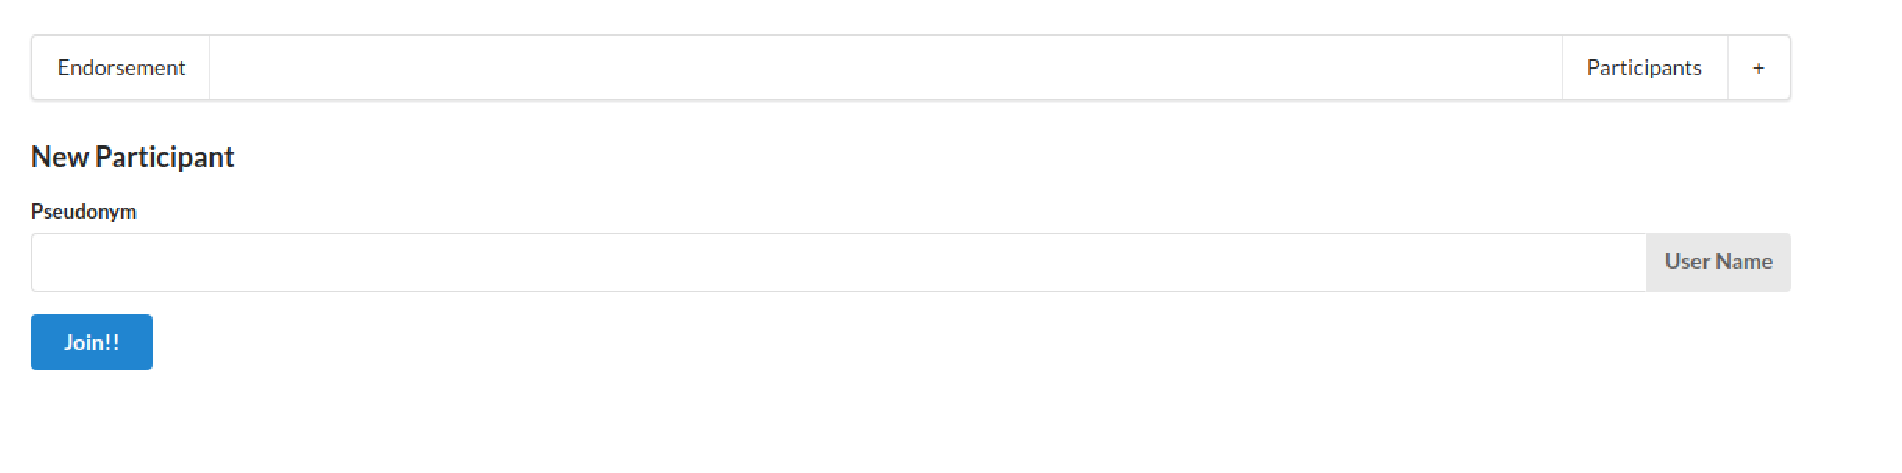
\includegraphics[width=0.95\textwidth]{Images/2_Frontend_JoinNetwork.eps} 
%%		\caption{Join Network using Pseudonym} 
%%		\label{joinNetwork}
%%	\end{figure}
%%	\item Send and Remove Endorsement: Anyone can view the details of all
%%		registered participants on the network which is a requirement mentioned
%%		by R3, R4. However, sending and removing endorsement checks if the
%%		message sender is a registered participant or not. Only if it's true,
%%		then the sending or removing of endorsement is called without error.
%%		This feature refers to requirement R1 and R2. Figure ~\ref{viewDetails}
%%		shows the view details of participants along with the send and remove
%%		endorsement feature.
%%		\begin{figure}[h]
%%			\includegraphics[width=0.95\textwidth]{Images/3_Frontend_ViewDetails.eps} 
%%			\caption{View Details of participants and endorse them} 
%%			\label{viewDetails}
%%	\end{figure}
%%\end{itemize}
%%
%%\section{Generalization} \label{sec:generalization}
%%The endorsement PoC is a general model that aggregates and assign reputation
%%scores to individuals based on their interaction in a network. As such, any
%%transactional network, e-commerce, content-serving platform, etc. can use it.
%%The platform-specific reputation system can still co-exist alongside the
%%endorsement model. It is useful to get an objective measure of the actual
%%transaction feedback(history, quality of services, etc.).  Consider a buy/sell
%%system scenario where two unknown entites, A and B are attempting to transact
%%with each other. The entities can check each other's rating/feedback from the
%%platform's reputation system in use. If that is not enough for deciding on the
%%transaction, they can check the endorsement network for the global reputation
%%score of the entity in question. As such, the decision is no more reliant only
%%on A's reputation or the platform's reputation. There is a third option that
%%guarantees a reliable and immutable data stored in a decentralized manner. From
%%the view of the platform, say, B/S, it allows users on endorsement network to
%%transact on B/S. The users of B/S gets output from decentralized trust score
%%storage system. The platform itself provides input to the endorsement system in
%%case of a failed transaction outcome to help penalize the peer in the
%%endorsement network. Doing so increases the accuracy in both systems. 
%%
%%
%%%The results presented in Chapter 4 are discussed and analyzed, including comments and reflections from the author. It may include the following: Comparison of obtained results with discussion,interpretation and evaluation of results. Results of analysis or modeling are described. Interpretations are drawn and connected to previous work
